\documentclass{article}

\usepackage{arxiv}

\usepackage[utf8]{inputenc} % allow utf-8 input
\usepackage[T1]{fontenc}    % use 8-bit T1 fonts
\usepackage{hyperref}       % hyperlinks
\usepackage{url}            % simple URL typesetting
\usepackage{booktabs}       % professional-quality tables
\usepackage{amsfonts}       % blackboard math symbols
\usepackage{nicefrac}       % compact symbols for 1/2, etc.
\usepackage{microtype}      % microtypography
\usepackage{lipsum}

\title{Improving Outcome Predictions for Patients Receiving Mechanical
Circulatory Support by Optimizing Imputation of Missing Values}

\author{
    Byron C. Jaeger
    \thanks{Source code available at
\url{https://github.com/bcjaeger/INTERMACS-missing-data}}
   \\
    Department of Biostatistics \\
    University of Alabama at Birmingham \\
  Birmingham, AL \\
  \texttt{\href{mailto:bcjaeger@uab.edu}{\nolinkurl{bcjaeger@uab.edu}}} \\
   \And
    Ryan Cantor, PhD
   \\
    University of Alabama at Birmingham \\
  Birmingham, AL \\
  \texttt{} \\
   \And
    Venkata Sthanam, MS
   \\
    University of Alabama at Birmingham \\
  Birmingham, AL \\
  \texttt{} \\
   \And
    Rongbing Xie, DrPH
   \\
    University of Alabama at Birmingham \\
  Birmingham, AL \\
  \texttt{} \\
   \And
    James K. Kirklin, MD
   \\
    University of Alabama at Birmingham \\
  Birmingham, AL \\
  \texttt{} \\
   \And
    Ramaraju Rudraraju, PhD
   \\
    University of Alabama at Birmingham \\
  Birmingham, AL \\
  \texttt{\href{mailto:ramaraju@uab.edu}{\nolinkurl{ramaraju@uab.edu}}} \\
  }


\begin{document}
\maketitle

\def\tightlist{}


\begin{abstract}
\textbf{Background} Risk prediction models play an important role in
clinical decision making. When developing risk prediction models,
practitioners often impute missing values to the mean. We evaluated the
impact of applying other strategies to impute missing values on the
prognostic accuracy of downstream risk prediction models, i.e., models
fitted to the imputed data. A secondary objective was to compare the
accuracy of imputation methods based on artificially induced missing
values. To complete these objectives, we used data from the Interagency
Registry for Mechanically Assisted Circulatory Support (INTERMACS).
\newline\textbf{Methods and Results} We applied twelve imputation
strategies in combination with two different modeling strategies for
mortality and transplant risk prediction following surgery to receive
mechanical circulatory support. Model performance was evaluated using
Monte-Carlo cross validation and measured based on outcomes 6-months
following surgery using the scaled Brier score, concordance index, and
calibration error. We used Bayesian hierarchical models to compare model
performance. Multiple imputation with random forests emerged as a robust
strategy to impute missing values, increasing model concordance by 0.003
(25th, 75th percentile: 0.008, 0.052) compared with imputation to the
mean for mortality risk prediction using a downstream proportional
hazards model. The posterior probability that single and multiple
imputation using random forests would improve concordance versus mean
imputation was 0.482 and 0.962, respectively.
\newline\textbf{Conclusion} Selecting an optimal strategy to impute
missing values and applying multiple imputation can improve the
prognostic accuracy of downstream risk prediction models.
\end{abstract}

\keywords{
    Missing Data
   \and
    INTERMACS
   \and
    imputation
   \and
    heart failure
   \and
    mortality
   \and
    risk prediction
  }

\hypertarget{introduction}{%
\section{Introduction}\label{introduction}}

\label{sec:introduction}

\linenumbers
\doublespacing

Heart disease is a leading cause of death in the United States. Heart
failure, a primary component of heart disease, affects over 6 million
Americans, and for \textasciitilde10\% of these patients medical
management is no longer effective
\cite{benjamin2017heart,national2017health}. Mechanical circulatory
support (MCS) is a surgical intervention in which a mechanical device is
implanted in parallel to the heart to improve circulation
\cite{patel2014contemporary}. Typically, MCS is used while a patient
waits for a heart transplant (bridge-to-transplant) or in some cases as
an alternative to transplant (destination therapy)
\cite{slaughter2009advanced}. Over 250,000 patients could benefit from
MCS \cite{miller2011left}. However, less than 4,000 new patients receive
a long-term MCS device each year, with widely heterogeneous outcomes
\cite{stewart2011keeping}. The 2-year survival probability on MCS ranges
from 61\% for destination therapy to 78\% for bridge-to-transplant
\cite{patel2014contemporary}. Reliable predictions of patient-specific
risk to experience key outcomes such as mortality or transplant after
receiving MCS can help improve patient selection, inform the design of
next generation pumps, and improve patient care strategies.

The Interagency Registry for Mechanically Assisted Circulatory Support
(INTERMACS) was launched to improve MCS patient outcomes through the
collection of patient characteristics, medical events, and long terms
outcomes at a nation wide level. Currently, INTERMACS comprises over
20,000 patients who have received a MCS device. As the largest registry
for data on patients receiving MCS devices, INTERMACS has been leveraged
to develop numerous risk prediction models for mortality and other types
of adverse events that may occur after receiving a device
\cite{hsich2012should, cotts2014predictors, eckman2011survival, kirklin2017eighth, kormos2019society, Adamo950}.
A critical step for developing risk prediction models is handling
missing data, which is common in a ``real world'' database that is not
designed for the rigor of data completeness found in a clinical trial.
While some missing values are related to data entry error, others may
relate to instability of a patient's circulatory status at the time of
implant. For instance, hemodynamic laboratory values are missing for
patients in whom invasive catheterizations were not performed. Patients
without invasive catheterizations may be too ill (unstable) to tolerate
the procedure. Instead, such patients may, after determination of basic
hemodynamics, proceed directly to device placement.

The primary aim of this article is to quantify how much the prognostic
value of a risk prediction model developed from the INTERMACS registry
depends on the strategy that was applied to impute missing data prior to
developing the model. A secondary aim is to measure imputation accuracy
of each strategy by introducing varying levels of artificial missing
data and then imputing it. Because imputation to the mean has been a
standard method for multiple annual summaries of the INTERMACS data, we
measure the potential improvement in prognostic value of a risk
prediction model when other strategies are applied to impute missing
data \emph{instead of imputation to the mean}. The over-arching aim is
to clarify which imputation strategies are most likely to improve risk
prediction (and by extension, quality of care) for patients who receive
MCS devices. This investigation can directly inform future analyses of
INTERMACS data and provide evidence quantifying the benefit of imputing
missing data with sound methodology.

\hypertarget{methods}{%
\section{Methods}\label{methods}}

\label{sec:methods}

\hypertarget{intermacs-registry}{%
\subsection{INTERMACS Registry}\label{intermacs-registry}}

\label{subsec:intermacs}

INTERMACS is a North American observational registry for patients
receiving MCS devices that began as a partnership between the National
Heart, Lung, and Blood Institute, US Food and Drug Administration, the
Centers for Medicaid and Medicare Services, industry, and individual
hospitals with the mission of improving MCS outcomes. In 2018, INTERMACS
became an official Society of Thoracic Surgeons database.

The current analysis was conducted using publicly available data
provided by the National Heart, Lung, and Blood Institute (see
\url{https://biolincc.nhlbi.nih.gov/studies/intermacs/}). We included a
contemporary cohort of 14,738 patients who received continuous flow LVAD
from 2012-2017. This is a secondary analysis of de-identified data
obtained from the National Heart Lung and Blood Institute. Primary data
collection is approved through University of Alabama Institutional
Review Board and at individual sites.

\hypertarget{outcomes-and-predictors}{%
\subsection{Outcomes and Predictors}\label{outcomes-and-predictors}}

Patient follow-up begins after implantation of a durable, long term MCS
device and continues while the device is in place. Registry endpoints
include death on a device, heart transplantation, or cessation of
support (for recovery and non-recovery reasons). Mortality and
transplant after MCS were the primary outcomes for the current study. As
there were only 310 cessation of support events, we did not analyze this
outcome. For mortality and transplant risk prediction models, we applied
cause-specific analysis to account for competing risks. For example, in
risk prediction models for mortality, patients were censored at time of
loss to follow-up, transplant, or cessation of support, whichever
occurred first. INTERMACS collects pre-implant data on patient
characteristics, medical status, and laboratory values. INTERMACS also
collects follow-up data at regularly scheduled visits and at occurrence
of adverse events such as re-hospitalization. For the current analysis,
all pre-implant variables were considered as potential predictors.

\hypertarget{statistical-inference-and-learning-with-missing-data}{%
\subsection{Statistical Inference and Learning with Missing
data}\label{statistical-inference-and-learning-with-missing-data}}

\label{subsec:inference_and_learning}

\paragraph{Statistical Inference}

To conduct statistical inference in the context of missing data setting,
analysts often create multiple imputed datasets, replicate an analysis
in each of them, and then pool their results to obtain valid test
statistics for hypothesis testing \cite{rubin2004multiple}. Imputation
strategies that create a single imputed dataset
(\textit{e.g., }imputation to the mean) have been shown to increase type
I errors (\textit{i.e., }rejecting a true null hypothesis) for
inferential statistics by artificially reducing the variance of observed
data and ignoring the uncertainty attributed to missing values
\cite{van2018flexible}. To ensure valid inference, imputation models
should leverage outcome variables to predict missing predictors
\cite{sterne2009multiple}. When very few data are missing, analysts may
apply listwise deletion, \textit{i.e., }removing any observation with at
least one missing value. However, listwise deletion can easily lead to
biased inference \cite{van2020rebutting}.

\paragraph{Statistical Learning}

In the presence of missing data, the goal of supervised statistical
learning is to develop a prediction function for an outcome variable
that accurately generalizes to testing data, which may or may not
contain missing values \cite{hastie2009elements}. Because testing data
may contain missing values, listwise deletion is not a feasible strategy
for statistical learning tasks. In contrast to statistical inference,
strategies that create a single imputed dataset are often used for
statistical learning \cite{kuhn2019feature}. Previous work has
emphasized the importance of imputation strategies with greater
accuracy, suggesting that more accurate imputation strategies lead to
better performance of downstream models (\textit{i.e., }models fitted to
the imputed data) \cite{jerez2010missing}. Others have shown that
imputation to the mean, model-based imputation, and multiple imputation
can provide Bayes-optimal prediction models provided certain assumptions
are true, but these assumptions are difficult to validate in applied
settings \cite{josse2019consistency}.

\paragraph{Using outcomes during imputation}

The outcome variable should be used to impute predictor values for
statistical inference, but using outcome variables for this purpose in
supervised learning can have unintended consequences in model
implementation. For instance, suppose we seek to predict an outcome
\(Y\) for a patient in the clinical setting. If the patient is missing
information for a predictor \(X\) and our model's strategy to impute
missing values of \(X\) leverages the observed value of \(Y\), how
should we impute \(X\)? If we do not already know \(Y\), then we cannot
impute \(X\) and hence cannot generate a valid prediction. On the other
hand, if we already know \(Y\), then we do not need to predict it. Due
to these practical considerations and because INTERMACS is often
leveraged to create prediction models for clinical practice
\cite{thomas2014pre}, we did not leverage outcome variables to impute
missing values of predictors in the current analysis.

\hypertarget{missing-data-strategies}{%
\subsection{Missing Data Strategies}\label{missing-data-strategies}}

\label{subsec:imputation}

\paragraph{Single and multiple imputation}

Several of the imputation methods we considered allowed for creation of
single or multiple imputed datasets. For downstream models fitted to
multiple sets of imputed data, we applied the modeling technique to each
imputed training set, separately, and then used a pooling technique to
generate a single set of predictions based on multiple imputed testing
data. Specifically, we created 10 imputed training and testing sets,
then applied a modeling procedure to each imputed training set and
computed model predictions on the corresponding imputed testing set,
which led to 10 sets of predictions. To aggregate these predictions, we
computed the median for each patient. Informal experiments where the
mean was used instead of the median to aggregate predictions showed
little or no difference in the model's prediction accuracy.

\paragraph{Imputation to the mean}

Imputing data to the mean involves three steps. First, numeric and
nominal variables are identified. Second, for each numeric variable, the
mean is computed and used to impute missing values in the corresponding
variable. Third, for each nominal variable, the mode is computed
(because one cannot compute a mean for categorical variables) and used
to impute missing values in the corresponding variable. The computed
means and modes are then stored for future imputation of testing data.
Because imputation to the mean is frequently used in practice, we use it
as a reference for comparison of all other strategies to impute missing
values.

\paragraph{Bayesian Regression}

Imputation with Bayesian regression draws imputed values from the
posterior distribution of model parameters, accounting for uncertainty
in both model error and estimation \cite{rubin2004multiple}. Multiple
imputation with chained equations (MICE), a well known technique for
generating multiply imputed data
\cite{azur2011multiple, van2018flexible, van2006fully}. In each
iteration of MICE, each specified variable in the dataset is imputed
using other variables in the dataset. These iterations are run until
convergence criteria have been met.

\paragraph{Predictive Mean Matching (PMM)}

PMM computes predicted values from a pre-specified model that treats one
incomplete column in the data, \(X\), as a dependent variable. For each
missing value in \(X\), PMM identifies a set of candidate donors based
on distance in predicted values of \(X\) \cite{landerman1997empirical}.
One donor is randomly drawn from the candidates, and the observed value
of the donor is taken to replace the missing value. When missing values
were imputed using PMM, we applied MICE to form multiple imputed
datasets. For consistency with other approaches, we also generated a
single imputed dataset using PMM by randomly selecting one of the
multiple datasets imputed.

\paragraph{K-Nearest-Neighbors (KNN)}

KNN imputation identifies \(k\) `similar' observations
(\textit{i.e., }neighbors) for each observation with a missing value in
a given variable \cite{chen2000nearest}. A donor value for the current
missing value is generated by sampling or aggregating the values from
the \(k\) nearest neighbors. In the current analysis, we identified 10
nearest neighbors using Gower's distance \cite{gower}. When imputing a
single dataset using KNN, we aggregated values from 10 nearest neighbors
using the median for numeric variables and the mode for categorical
variables. When imputing multiple datasets using KNN, we aggregated
values from 2, 6, 11, 16, and 20 neighbors, separately, to create 5
imputed datasets.

\paragraph{Hot Deck}

Similar to KNN, hot deck imputation finds \(k\) similar observations for
each observation with a missing value in a given variable
\cite{andridge2010hotdeck}. However, hot deck imputation uses a less
computationally intensive approach, either identifying neighbors at
random or using a subset of variables to find similar observations. When
imputing a single dataset using hot deck imputation, we used a selection
of 5 variables simultaneously to identify nearest neighbors. When
imputing multiple datasets using hot deck imputation, we used a separate
numeric variable for each dataset.

\paragraph{Random forests}

Random forests grow an ensemble of de-correlated decision trees, where
each tree is grown using a bootstrapped replicate of the original
training data
\cite{Breiman2001, hothorn2006survival, strobl2007bias, strobl2008conditional, ishwaran2008random, jaeger2019oblique}.
A particularly helpful feature of random forests is their ability to
estimate testing error by aggregating each decision tree's prediction
error on data outside of their bootstrapped sample
(\textit{i.e., }out-of-bag error). In the current analysis, we conduct
MICE using one random forest to impute each variable, separately. For
each imputed dataset, we allowed random forests to be re-fitted until
out-of-bag error stabilized or a maximum number of iterations was
completed. When imputing a single dataset, we used 250 trees per forest
and a maximum of 10 iterations. When imputing multiple datasets, we used
50 trees per forest and applied PMM using the random forest's predicted
values to impute missing data by sampling one value from a pool of 10
potential donors.

\paragraph{Missingness incorporated as an attribute (MIA)}

MIA is a technique that uses missing status as a predictor rather than
explicitly imputing missing values
\cite{twala2009empirical, ding2010investigation}. MIA adds another
category to nominal variables: ``Missing''. For numeric variables, MIA
creates two columns: one where missing values are imputed with positive
infinity and the other with negative infinity. Since PH models are not
compatible with infinite values, we only use MIA in boosting models.
When a decision tree uses a finite cut-point to split a given numeric
variable, it will assess the cut-point using both the positive and
negative infinite imputed columns, and utilize whichever column provides
the best split of the current data. This procedure translates to sending
all missing values to the left or to the right when forming two new
nodes of the decision tree, using whichever direction results in a
better split.

\paragraph{Assumptions}

Each missing data strategy poses different assumptions regarding the
data and the mechanisms that lead to missing values in the data.
Imputation using Bayesian regression makes the same distributional
assumptions as the Bayesian models that are applied. The
\texttt{miceRanger} algorithm does not make any formal distributional
assumptions, as random forests are non-parametric and can thus handle
skewed and multi-modal data as well as categorical data that are ordinal
or non-ordinal. Hot deck and KNN imputation also do not make
distributional assumptions, but implicitly assume that a missing value
for a given observation can be approximated by aggregating observed
values from the \(k\) most similar observations. PMM makes a similar
implicit assumption, but is slightly more robust to skewed or
multi-modal data because imputed values are sampled directly from
observed ones. MIA operates based on an implicit assumption that
missingness itself is informative. It is difficult to validate these
assumptions in applied settings and also likely that downstream models
will perform poorly if an imputation technique's assumptions are
invalid.

\hypertarget{evaluating-imputation-accuracy}{%
\subsection{Evaluating Imputation
Accuracy}\label{evaluating-imputation-accuracy}}

\label{subsec:imputation_accuracy}

Imputation accuracy was computed for each numerical and nominal
variable, separately. Numeric variable imputation accuracy was measured
using a re-scaled mean-squared error:
\[1 - \frac{\textrm{MSE}(\textrm{current imputation method})}{\textrm{MSE}(\textrm{imputation to the mean})}.\]
This score is greater than 0 if
\(\textrm{MSE}(\textrm{current imputation method})\) is smaller than
\(\textrm{MSE}(\textrm{imputation to the mean})\), equal to 0 if the two
MSEs are equal, and less than 0 if
\(\textrm{MSE}(\textrm{current imputation method})\) is greater than
\(\textrm{MSE}(\textrm{imputation to the mean})\). Nominal variable
imputation accuracy was measured using a re-scaled classification
accuracy:
\[1 - \frac{\textrm{Classification error}(\textrm{current imputation method})}{\textrm{Classification error}(\textrm{imputation to the mean})}.\]
This score is greater than 0 if the classification error of the current
imputation method is less than that of imputation to the mean, equal to
0 if the two classification errors are equal, and less than 0 of the
classification error of the current imputation method is worse than
imputation to the mean. These numeric and nominal scores are analogous
to the more well known \(R^2\) and Kappa statistics, respectively, but
are modified slightly in the current analysis so that imputation to the
mean will always have a score of 0. This modification makes it easier to
compare the accuracy of each imputation strategy directly with that of
imputation to the mean.

\hypertarget{risk-prediction-models}{%
\subsection{Risk Prediction Models}\label{risk-prediction-models}}

\label{subsec:modeling}

We applied two modeling strategies after imputing missing values:

\begin{itemize}
\tightlist
\item
  Cox proportional hazards (PH) model with forward stepwise variable
  selection
\item
  Gradient boosted decision trees (hereafter referred to as `boosting')
\end{itemize}

A thorough description of stepwise variable selection and boosting can
be found in Sections 6.1.2 and 8.2.2, respectively, of
\emph{Introduction to Statistical Learning}
\cite{james2013introduction}. Sir David Cox's PH model is one of the
most frequently applied methods for the analysis of right-censored
time-to-event outcomes \cite{kleinbaum2010survival}. According to the PH
assumption, the effect of a unit increase in a predictor is
multiplicative with respect to a baseline hazard function. Boosting
grows a sequence of decision trees, each using information from the
previous trees in an attempt to correct their errors
\cite{friedman2001greedy, chen2016xgboost}.

\hypertarget{evaluation-of-predictions}{%
\subsection{Evaluation of Predictions}\label{evaluation-of-predictions}}

\label{subsec:evaluation}

\paragraph{The Brier score}

The prognostic value of each risk prediction model was primarily
assessed using the Brier score, which depends on both the discrimination
and calibration of predicted risk values
\cite{graf1999assessment, rufibach2010use}. Let \(\tilde{Y}_i(t)\)
represent the observed status of individual \(i\) at time \(t > 0\) in a
testing set of \(M\) observations. Suppose \(\tilde{Y}_i(t)=1\) if there
is an observed event at or before \(t\) and \(\tilde{Y}_i(t)=0\)
otherwise. The Brier score is computed with
\begin{equation} \label{eqn:brier_score}
\widehat{\textrm{BS}}(t)= \frac{1}{M} \sum_{i=1}^{M} \widehat{W}_i(t) \left\{ \tilde{Y}_i(t) - \widehat{S}(t \mid \bm{x}_i) \right\}^2, \end{equation}
where, for the \(i^{th}\) observation, \(\widehat{S}(t \mid \bm{x}_i)\)
is the estimated probability of survival at time \(t\) according to a
given risk prediction model, \(\bm{x}_i\) is the set of input values for
predictor variables in the model, and \(\widehat{W}_i(t)\) is the
inverse proportional censoring weight at time \(t\)
\cite{gerds2006consistent}. Thus, the Brier score is the mean squared
difference between observed event status and expected event status
according to a RPE at time \(t\). Throughout the current analysis, we
set \(t = 6\) months after receiving MCS to focus on short term risk
prediction. Models have been developed to simultaneously predict short
term and long term mortality risk after receiving MCS, but these are
beyond the scope of the current study
\cite{blackstone1986decomposition}.

\paragraph{The scaled Brier score}

The Brier score is dependent on the rate of observed events, which can
make it a difficult metric to interpret. It is often more informative to
scale the Brier score based on the Brier score of a naive model. More
specifically, for a given risk prediction model, the scaled Brier score
is computed as
\[\textrm{Scaled } \widehat{\textrm{BS}}(t)\textrm{ of model } = 1 - \frac{\widehat{\textrm{BS}}(t)\textrm{ of model}}{\widehat{\textrm{BS}}(t)\textrm{ of naive model}}.\]
As the Brier score for risk prediction is analogous to mean-squared
error for prediction of a continuous outcome, the scaled Brier score is
analogous to the \(R^2\) statistic. Similar to the \(R^2\) statistic, a
scaled \(\widehat{\textrm{BS}}(t)\) of 1.00 and 0.00 indicate a perfect
and worthless model, respectively. In our analyses, a Kaplan-Meier
estimate based on the training data (\textit{i.e., }a risk prediction
model that did not use any predictor variables) provided the naive
prediction. In the current analysis, we multiply scaled Brier score
values by 100 for ease of interpretation.

\paragraph{Discrimination and calibration}

The discrimination of a risk prediction model measures the probability
that the model will successfully identify which of two observations is
at higher risk for the event of interest. We estimated discrimination
using a time-dependent concordance (C-) index that accounted for
covariate-dependent censoring. A C-index of 0.50 and 1.00 correspond to
worthless and perfect discrimination, respectively. Similar to the
scaled Brier score, we multiply C-index values by 100 for ease of
interpretation. Calibration slope plots measure a risk prediction
model's absolute accuracy. We estimated calibration error by averaging
the squared distance between expected and observed event rates according
to a calibration plot. Full description of these evaluation metrics are
available \cite{gerds2014calibration, gerds2013estimating}.

\hypertarget{internal-validation-via-monte-carlo-cross-validation-mccv}{%
\subsection{Internal Validation via Monte-Carlo Cross-Validation
(MCCV)}\label{internal-validation-via-monte-carlo-cross-validation-mccv}}

\label{subsec:internal}

To assess the prognostic value of each missing data strategy, we
internally validated a total of 23 modeling algorithm based on
combinations of imputation strategies and modeling strategies described
in Sections \ref{subsec:imputation} and \ref{subsec:modeling}. For
convenience, we use the term `modeling algorithm' to denote the
combination of a missing data strategy and a modeling strategy
(\textit{e.g., }imputation using mean/mode values followed by fitting
the PH model with stepwise variable selection) \cite{kuhn2013applied}.
We conducted internal validation using 200 replicates of Monte-Carlo
cross validation, a resampling technique for internal validation.

\paragraph{Steps taken in each replicate}

In each replicate of Monte-Carlo cross validation, 50\% of the available
data were used for model training and testing. All predictor variables
with \textless{} 50\% missing values were considered for imputation and
subsequent model development. Among these variables, artificial
missingness (0\%, 15\%, or 30\% additional missing values) was induced
based on patient age, with younger and older patients more likely to
have missing data compared to patients who were between 40 and 65 years
of age. Prior to imputation, 50 predictor variables were selected using
a boosting model that quantified variable importance as the fractional
contribution of each predictor to the model based on the total gain
attributed to using the predictor while growing decision trees.
Imputation was conducted in the training and testing sets, separately,
for each imputation strategy. Although some imputation strategies
(\textit{e.g., }KNN and random forests) can impute data in the testing
set using models fitted to the training set, others
(\textit{e.g., }Bayesian regression, PMM, and hot deck) cannot.
Therefore, to ensure fair comparisons in our experiment, each imputation
procedure imputed data in the training set using models fitted to the
training set and then imputed data in the testing set using models
fitted to the testing set. After imputation, Cox PH and boosting models
were applied to each imputed dataset, separately. Last, model
predictions for death and transplant were computed at 6 months following
MCS surgery.

\paragraph{Bayesian analysis of model performance}

To determine whether any of the imputation methods described above had
improved upon imputation to the mean, we applied Bayesian hierarchical
models to analyze differences in scaled Brier score
\cite{benavoli2017time}. This strategy provides a flexible framework to
conduct hypothesis testing and also accounts for correlation occurring
within each replicate of Monte-Carlo cross validation. Specifically,
within each replicate of Monte-Carlo cross validation, the performance
of different modeling algorithms are correlated because they are trained
and tested using the same data.

\hypertarget{statistical-analysis}{%
\subsection{Statistical analysis}\label{statistical-analysis}}

Participant characteristics were tabulated for the overall population
and stratified by event status. Continuous and categorical variables
were summarized as mean (standard deviation) and percent, respectively.
The number and proportion of missing values were also tabulated for the
overall population and stratified by event status. Missing data patterns
were visualized for the overall population using an UpSet plot
\cite{lex2014upset}. All of the proceeding analyses were conducted using
resampling results from Monte-Carlo cross validation. Imputation
accuracy was aggregated for all numeric and nominal variables to create
two overall scores for each imputed dataset. For imputation methods that
created multiple datasets, scores were aggregated over each dataset to
provide a single summary score. The distribution
(\textit{i.e., }25\textsuperscript{th}, 50\textsuperscript{th}, and
75\textsuperscript{th} percentile) of the scaled Brier score was
estimated for each modeling algorithm.

We split our results from Monte-carlo cross validation into four
datasets based on outcome (mortality or transplant) and modeling
procedure (Cox PH or boosting). For each dataset, we fit one
hierarchical Bayesian model where the dependent variable was scaled
Brier score and independent variables included the imputation strategy
applied and the amount of artificially missing data (0\%, 15\%, or 30\%)
induced before imputation. With each model, we estimated the difference
in scaled Brier score of downstream models when random forests, Bayesian
regression, PMM, hot deck, MIA, or KNN imputation were applied to impute
missing values instead of imputation to the mean.

\hypertarget{computational-details}{%
\subsection{Computational Details}\label{computational-details}}

\label{subsec:computing}

SAS software (version 9.4) and Python (version 3.8.2) were used to
create analytic data for the current study
\cite{van1995python, sas2013}. Base R (version 4.0.3) was used in
combination with a number of open-source R packages
(\textit{e.g., }\texttt{drake}, \texttt{tidyverse}, \texttt{naniar},
\texttt{table.glue}, \texttt{mice}, \texttt{miceRanger}, and others) to
conduct our analysis
\cite{drake, naniar, mice, miceRanger, table.glue, tidyverse, rstanarm, tidybayes, survival, tidymodels, riskRegression}.
Our R code is available on GitHub (see
\url{https://github.com/bcjaeger/INTERMACS-missing-data})
\cite{byron_2020_4247449}. We used Cheaha, a high performance computing
cluster at University of Alabama at Birmingham, to perform the 200
Monte-Carlo cross validation runs \cite{cheaha}.

\hypertarget{results}{%
\section{Results}\label{results}}

\paragraph{Patient Characteristics}

During the first 6 months after receiving MCS, the number (\% of overall
population) of deaths, transplants, and loss-to-follow-up events was
1,897 (13\%), 1,067 (7.2\%), and 981 (6.7\%), respectively. The mean
(standard deviation) age of patients was 57 (13) years, 66\% of patients
identified as white and 79\% were male (Table
\ref{tbl_characteristics}).

\paragraph{Missing data}

Many predictor variables exhibited similar proportions of missing values
in different outcome groups (Table \ref{tbl_missingness}). However, the
number (percent) of missing values for surgery time was an exception,
with 6,125 (41.6\%) in the overall population, 2,246 (53.4\%) among
patients who died, and 1,713 (27.2\%) among patients who were censored.
Additionally, missing values for surgery time were frequently
accompanied by missing values for CV pressure (Figure \ref{fig:upset}).

\paragraph{Imputation accuracy}

Single imputation strategies were more accurate than their counterparts
using multiple imputation in 8 out of 10 comparisons of nominal scores
and 10 out of 10 comparisons of numeric scores (Table
\ref{tbl_impute_accuracy}). When an additional 15\% of data were
missing, single imputation KNN obtained the highest nominal accuracy
(score: +0.02, 95\% CI -0.05, 0.15) and single imputation with random
forests obtained the highest numeric accuracy (score: +0.05, 95\% CI
0.03, 0.08). When an additional 30\% of data were missing, imputation to
the mean obtained the highest numeric and nominal scores.

\hypertarget{scaled-brier-score}{%
\subsection{Scaled Brier score}\label{scaled-brier-score}}

\paragraph{Mortality risk prediction}

When no additional data were amputed and imputation to the mean was
applied before fitting risk prediction models, the median
(25\textsuperscript{th}, 75\textsuperscript{th} percentile) scaled Brier
score was 6.09 (5.71, 6.54) for Cox PH and 7.27 (6.83, 7.77) for
boosting models (Table \ref{tbl_md_strat_dead_ipa}; top panel). Multiple
imputation strategies universally obtained higher scaled Brier scores
versus their single imputation counterparts. Multiple imputation using
random forests provided the highest scaled Brier score compared to other
strategies, leading to a median (25\textsuperscript{th},
75\textsuperscript{th} percentile) increase in the scaled Brier score of
0.34 (0.12, 0.54) for Cox PH and 0.34 (0.14, 0.58) for boosting models.
These performance increments improved when an aditional 15\% and 30\% of
data were amputed (Table \ref{tbl_md_strat_dead_ipa}; middle and bottom
panel).

\paragraph{Transplant risk prediction}

When no additional data were amputed and imputation to the mean was
applied before fitting risk prediction models, the median
(25\textsuperscript{th}, 75\textsuperscript{th} percentile) scaled Brier
score was 9.35 (8.80, 9.71) for Cox PH and 9.00 (8.55, 9.41) for
boosting models (Table \ref{tbl_md_strat_txpl_ipa}; top panel). For Cox
PH models, imputation to the mean provided the lowest scaled Brier
score, and random forest imputation led to a median
(25\textsuperscript{th}, 75\textsuperscript{th} percentile) increase of
0.13 (0.03, 0.29) versus imputation to the mean. For boosting models,
surprisingly, imputation to the mean provided a higher scaled Brier
score than all imputation methods except for multiple imputation using
Bayesian regression. When an additional 15\% and 30\% of data were
amputed, the performance increments corresponding to the use of multiple
imputation increased for both Cox PH and boosting models (Table
\ref{tbl_md_strat_txpl_ipa}; middle and bottom panel).

\hypertarget{discrimination-and-calibration}{%
\subsection{Discrimination and
calibration}\label{discrimination-and-calibration}}

\paragraph{Mortality risk prediction}

Regardless of how much additional data were amputed, boosting models
obtained higher median C-indices than PH models for prediction of
6-month mortality risk (Table \ref{tbl_md_strat_dead_auc}). In addition,
all models that used multiple imputation consistently obtained higher
median C-indices compared to their counterparts using single imputation.
When 0 and 15\% additional data were amputed, median calibration error
was lower for PH models compared to boosting models, but boosting models
obtained lower median calibration error when 30\% additional data were
amputed (Table \ref{tbl_md_strat_dead_cal_error}). Almost all imputation
strategies provided lower median calibration error compared with
imputation to the mean.

\paragraph{Transplant risk prediction}

For all amounts of additional data amputed, PH models obtained higher
median C-indices than boosting models for prediction of 6-month
transplant risk (Table \ref{tbl_md_strat_txpl_auc}). Similar to
mortality risk prediction, multiple imputation strategies generally
provided higher C-indices than their counterparts using single
imputation strategy. For boosting models, MIA provided higher C-indices
compared to all other single imputation strategies and had similar or
superior performance compared to several multiple imputation strategies.
Differences in calibration error were minor when no additional missing
data were amputed (Table \ref{tbl_md_strat_txpl_cal_error}). When an
additional 30\% of data were amputed, boosting models using MIA obtained
lower calibration error than any other strategy.

\hypertarget{bayesian-analysis-of-model-performance}{%
\subsection{Bayesian analysis of model
performance}\label{bayesian-analysis-of-model-performance}}

Adjusting for the amount of additional missing data amputed and the
outcome variable, the posterior probability that an imputation strategy
would improve the scaled Brier score of a downstream model relative to
imputation to the mean was maximized by using multiple imputation with
random forests (probability of improvement: 1.000; Figure
\ref{fig:fig_md_strat_infer_ipa}). Similarly, multiple imputation using
random forests was estimated to have the highest posterior probability
of improving the C-index in comparison to using imputation to the mean
(probability of improvement: 1.000; Figure
\ref{fig:fig_md_strat_infer_auc}). However, the estimated posterior
probability of a reduction in calibration was 1 when using either single
or multiple imputation with random forests compared with imputation to
the mean (Figure \ref{fig:fig_md_strat_infer_cal_error}). Although
imputation using random forest was estimated to be the best overall
option, there was moderate to strong evidence that MIA and each multiple
imputation strategy we applied would improve prognostic accuracy of
downstream models compared with imputation to the mean.

\hypertarget{discussion}{%
\section{Discussion}\label{discussion}}

In this article, we leveraged INTERMACS registry data to evaluate how
the use of different imputation strategies prior to fitting a risk
prediction model would impact the external prognostic accuracy of the
model. External prognostic accuracy was measured at 6 months after
receiving MCS, and the primary measure of accuracy was the scaled Brier
score. We evaluated the performance of 12 imputation strategies in a
broad range of settings by varying (1) the amount of additional missing
data amputed prior to performing imputation, (2) the type of risk
prediction model applied after imputation, and (3) the outcome variable
for the risk prediction model. Our resampling experiment indicated that
conducting multiple imputation has a high likelihood of increasing the
downstream scaled Brier score and C-index of risk prediction models
compared with imputation to the mean. Additionally, multiple imputation
with random forests emerged as the imputation strategy that maximized
the probability of developing a more prognostic model compared with
imputation to the mean.

In previous studies involving the INTERMACS data registry, imputation to
the mean has been applied prior to developing a mortality risk
prediction model
\cite{hsich2012should, cotts2014predictors, eckman2011survival, kirklin2017eighth, kormos2019society, Adamo950}.
An interesting recent study indicates that imputation to the mean can
provide an asymptotically consistent prediction model, given the
prediction model is flexible and non-linear \cite{josse2019consistency}.
However, theoretical results for finite samples have not yet been
established. Our results provide relevant data for the finite sample
case, suggesting that using imputation strategies considered in the
current study instead of imputation to the mean can improve the
prognostic accuracy of downstream models, particularly if multiple
imputation is applied. Imputation to the mean should be avoided in
future analyses of the INTERMACS registry and analyses where inflexible
models are applied.

Previous research has also established evidence in favor of applying
multiple imputation to improve the prognostic value of risk prediction
models. For example, Hassan and Atiya demonstrated superior downstream
prediction using an ensemble multiple imputation method on synthetic
data with continuous outcomes \cite{hassan2007regression}. Similarly,
Nanni et. al demonstrated superior performance in downstream prediction
when missing values were imputed using their proposed ensemble multiple
imputation method \cite{nanni2012classifier}. Notably, the authors
artificially induced missing values in these studies and the largest
real dataset that was evaluated contained less than 700 observations. An
article by Jerez et. al evaluated missing data strategies based on the
downstream task of fitting a neural network and predicting early breast
cancer relapse \cite{jerez2010missing}. The authors found that KNN
imputation led to risk prediction models with the highest discrimination
and lowest calibration error. Results from the current study are
consistent with these previous findings but also extend their results by
providing evidence from a larger source of data
(\textit{i.e., }INTERMACS) and dealing with `real-world' missing values.

Others have previously evaluated imputation techniques based on the
accuracy with which these techniques impute missing values in the
training data
\cite{tutz2015improved, little2013joys, steele2018machine}. While it is
intuitive to hypothesize that more accurate imputation will provide more
prognostic downstream models, our results do not support this
supposition. For example, when an additional 30\% of missing data were
amputed, none of the missing data strategies we implemented obtained
higher accuracy than imputation to the mean. However, using \emph{any}
of the multiple imputation strategies we considered instead of
imputation to the mean increased prognostic accuracy of downstream
models when an additional 30\% of missing data were amputed. This result
is likely explained by the bias variance tradeoff. In particular, single
imputation techniques may lead to prediction models with lower bias but
higher variance than multiple imputation techniques.

\paragraph{Strengths and limitations}

The current analysis has a number of strengths. We leveraged the
INTERMACS data registry, comprising one of the largest cohorts of
patients who received MCS. We applied a well known resampling method to
internally validate modeling algorithms for risk prediction. Last, we
made our analysis R code available in a public repository
(\url{https://github.com/bcjaeger/INTERMACS-missing-data}). Last, the
approach presented in this paper provides a general framework that can
be applied in other studies where missing data are imputed prior to
fitting a risk prediction model. The current analysis should also be
interpreted in the context of known limitations. We considered a small
subset of existing strategies to impute missing data, and other
strategies may have provided stronger improvements compared with
imputation to the mean. The models we studied obtained low values of
scaled Brier score, indicating low prediction accuracy. It is unclear
how results may vary for models with higher prediction accuracy. Also,
it was not feasible to use only the training data to impute missing
values in the testing data due to a lack of available software. Although
the \texttt{miceRanger} package allows imputation of new data using
existing models, few software packages for imputation allow users to
implement multiple imputation with this protocol. Future analyses should
introduce more flexible software and hands-on tutorials so that future
investigators can optimize imputation of missing data.

\paragraph{Conclusion}

Selecting an optimal strategy to impute missing values can impact the
prognostic accuracy of downstream risk prediction models. In the current
analysis, conducting multiple imputation using random forests emerged as
an optimal strategy to impute missing values in the INTERMACS data. This
investigation can directly inform future analyses of INTERMACS data and
provide evidence quantifying the benefit of imputing missing data with
sound methodology.

\clearpage
\begin{table}
\caption{Participant characteristics stratified by event status. The majority of patients were male and nearly all mechanical circulatory support devices were left-ventricular assistance devices.}
\label{tbl_characteristics}


\begin{tabular}{lccccc}
\toprule
Characteristic & Overall & Censored & Cessation of support & Dead & Transplant\\
\midrule
No. of patients & 14,738 & 6,308 & 310 & 4,204 & 3,916\\
Age, years & 57 (13) & 57 (13) & 48 (14) & 61 (12) & 53 (12)\\
Sex &  &  &  &  & \\
\hspace{1em}Female & 21 & 22 & 41 & 22 & 19\\
\hspace{1em}Male & 79 & 78 & 59 & 78 & 81\\
\addlinespace
Race &  &  &  &  & \\
\hspace{1em}White & 66 & 63 & 64 & 71 & 67\\
\hspace{1em}Black & 25 & 28 & 27 & 21 & 23\\
\hspace{1em}Other & 9.2 & 9.6 & 9.4 & 7.4 & 10\\
Body mass index & 29 (7) & 29 (7) & 29 (8) & 29 (7) & 28 (6)\\
\addlinespace
Device strategy &  &  &  &  & \\
\hspace{1em}Other & 0.6 & 0.6 & 2.6 & 0.5 & 0.6\\
\hspace{1em}Bridge to transplant & 52 & 43 & 51 & 40 & 81\\
\hspace{1em}Destination therapy & 47 & 56 & 46 & 60 & 18\\
LVEDD & 6.83 (1.10) & 6.85 (1.07) & 6.49 (0.93) & 6.69 (1.12) & 6.95 (1.12)\\
\addlinespace
Urinary albumin, g/dl & 3.41 (0.64) & 3.42 (0.61) & 3.41 (0.64) & 3.33 (0.66) & 3.49 (0.65)\\
Urinary creatinine, mg/dl & 1.39 (0.68) & 1.36 (0.62) & 1.17 (0.53) & 1.49 (0.77) & 1.35 (0.67)\\
CV pressure & 10.8 (6.2) & 10.4 (6.1) & 9.9 (6.0) & 11.6 (6.5) & 10.7 (6.0)\\
Periphal edema & 35 & 33 & 37 & 44 & 31\\
BUN, mg/dl & 29 (18) & 28 (17) & 22 (13) & 32 (19) & 28 (18)\\
\addlinespace
Bilirubin levels, mg/dl & 1.37 (1.84) & 1.25 (1.14) & 1.28 (1.95) & 1.52 (2.46) & 1.41 (1.97)\\
Device type &  &  &  &  & \\
\hspace{1em}Bi-ventricular assistance device & 3.5 & 2.1 & 0.3 & 5.8 & 3.4\\
\hspace{1em}Left-ventricular assistance device & 97 & 98 & 100 & 94 & 97\\
Surgery time, minutes & 292 (113) & 289 (110) & 272 (96) & 320 (128) & 272 (98)\\
\addlinespace
CPB time, minutes & 95 (49) & 93 (45) & 88 (38) & 103 (56) & 90 (44)\\
\bottomrule
\multicolumn{6}{l}{\rule{0pt}{1em}\textit{Note: }}\\
\multicolumn{6}{l}{\rule{0pt}{1em}Table values are mean (standard deviation) or \%}\\
\end{tabular}

\end{table}

\clearpage

\begin{table} 
 \caption{Number (percent) of missing values for a selection of predictor variables in the overall population and in subgroups based on event status. Many predictor variables exhibited similar proportions of missing values in different outcome groups, but surgery time was an exception.} 
\label{tbl_missingness} 
 
\begin{tabular}{lccccc}
\toprule
 & Overall & Dead & Transplant & Censored & Cessation of support \\ 
\midrule
CV pressure & 7,415 (50.3\%) & 2,156 (51.3\%) & 2,006 (51.2\%) & 3,108 (49.3\%) & 145 (46.8\%) \\ 
Surgery time, minutes & 6,125 (41.6\%) & 2,246 (53.4\%) & 2,007 (51.3\%) & 1,713 (27.2\%) & 159 (51.3\%) \\ 
Periphal edema & 5,093 (34.6\%) & 1,543 (36.7\%) & 1,470 (37.5\%) & 1,952 (30.9\%) & 128 (41.3\%) \\ 
LVEDD & 3,155 (21.4\%) & 1,000 (23.8\%) & 866 (22.1\%) & 1,233 (19.5\%) & 56 (18.1\%) \\ 
Urinary albumin, g/dl & 1,014 (6.88\%) & 326 (7.75\%) & 309 (7.89\%) & 359 (5.69\%) & 20 (6.45\%) \\ 
CPB time, minutes & 1,010 (6.85\%) & 287 (6.83\%) & 274 (7.00\%) & 421 (6.67\%) & 28 (9.03\%) \\ 
Bilirubin levels, mg/dl & 850 (5.77\%) & 291 (6.92\%) & 237 (6.05\%) & 304 (4.82\%) & 18 (5.81\%) \\ 
Body mass index & 77 (0.52\%) & 26 (0.62\%) & 19 (0.49\%) & 31 (0.49\%) & 1 (0.32\%) \\ 
BUN, mg/dl & 50 (0.34\%) & 10 (0.24\%) & 8 (0.20\%) & 32 (0.51\%) & 0 (0.00\%) \\ 
Sex & 24 (0.16\%) & 9 (0.21\%) & 4 (0.10\%) & 11 (0.17\%) & 0 (0.00\%) \\ 
Urinary creatinine, mg/dl & 20 (0.14\%) & 8 (0.19\%) & 4 (0.10\%) & 8 (0.13\%) & 0 (0.00\%) \\ 
Age, years & 0 (0.00\%) & 0 (0.00\%) & 0 (0.00\%) & 0 (0.00\%) & 0 (0.00\%) \\ 
Race & 0 (0.00\%) & 0 (0.00\%) & 0 (0.00\%) & 0 (0.00\%) & 0 (0.00\%) \\ 
Device strategy & 0 (0.00\%) & 0 (0.00\%) & 0 (0.00\%) & 0 (0.00\%) & 0 (0.00\%) \\ 
Device type & 0 (0.00\%) & 0 (0.00\%) & 0 (0.00\%) & 0 (0.00\%) & 0 (0.00\%) \\ 
\bottomrule
\end{tabular} 
 \end{table}

\clearpage

\begin{table} 
 \caption{Accuracy of strategies to impute artificial missing data. Table values are the median change in accuracy (25th, 75th percentile) relative to the accuracy of imputation to the mean. In general, multiple imputation strategies had lower accuracy than single imputation strategies, and few imputation strategies were more accurate than imputation to the mean.} 
\label{tbl_impute_accuracy} 
 
\begin{tabular}{lcccc}
\toprule
& \multicolumn{2}{c}{Nominal variables} & \multicolumn{2}{c}{Numeric variables} \\ 
 \cmidrule(lr){2-3}\cmidrule(lr){4-5}
 & Single imputation & Multiple imputation & Single imputation & Multiple imputation \\ 
\midrule
\multicolumn{1}{l}{+15\% additional missing data} \\ 
\midrule
Imputation to the mean & 0 (reference) & --- & 0 (reference) & --- \\ 
Hot deck & -0.24 (-0.34, -0.16) & -0.25 (-0.37, -0.18) & -0.35 (-0.53, -0.29) & -0.42 (-0.54, -0.36) \\ 
K-nearest-neighbors & +0.02 (-0.05, 0.15) & -0.01 (-0.09, 0.11) & +0.01 (-0.01, 0.03) & -0.02 (-0.05, 0.00) \\ 
Predictive mean matching & -0.15 (-0.34, 0.00) & -0.15 (-0.35, 0.00) & -0.25 (-0.40, -0.20) & -0.26 (-0.35, -0.21) \\ 
Random forest & -0.15 (-0.26, -0.03) & -0.15 (-0.26, -0.03) & +0.05 (0.03, 0.08) & +0.02 (-0.01, 0.04) \\ 
Bayesian regression & -0.14 (-0.26, 0.01) & -0.14 (-0.27, 0.01) & -0.30 (-0.41, -0.23) & -0.30 (-0.41, -0.23) \\ 
\midrule
\multicolumn{1}{l}{+30\% additional missing data} \\ 
\midrule
Imputation to the mean & 0 (reference) & --- & 0 (reference) & --- \\ 
Hot deck & -0.25 (-0.34, -0.18) & -0.26 (-0.36, -0.18) & -0.34 (-0.46, -0.30) & -0.40 (-0.53, -0.36) \\ 
K-nearest-neighbors & -0.04 (-0.09, 0.03) & -0.07 (-0.13, 0.00) & -0.02 (-0.03, -0.01) & -0.05 (-0.07, -0.04) \\ 
Predictive mean matching & -0.18 (-0.38, -0.04) & -0.18 (-0.37, -0.04) & -0.29 (-0.46, -0.24) & -0.29 (-0.40, -0.25) \\ 
Random forest & -0.18 (-0.28, -0.07) & -0.18 (-0.28, -0.08) & -0.01 (-0.03, 0.01) & -0.03 (-0.06, -0.01) \\ 
Bayesian regression & -0.17 (-0.29, -0.04) & -0.17 (-0.29, -0.05) & -0.31 (-0.43, -0.27) & -0.31 (-0.43, -0.27) \\ 
\bottomrule
\end{tabular} 
 \end{table}

\clearpage

\begin{table} 
 \caption{Median (25th, 75th percentile) change in scaled Brier score when different imputation strategies were applied to training and testing sets instead of imputation to the mean prior to developing a risk prediction model for mortality. Table values show the scaled Brier score for imputation to the mean. For other imputation strategies, table values show the change in scaled Brier score relative to the scaled Brier score when imputation to the mean was applied. All table values are multiplied by 100 for ease of interpretability. Multiple imputation with random forests leads to the highest scaled Brier score for both models and when 0\%, 15\%, or 30\% of additional data in the training and testing sets were set to missing.} 
\label{tbl_md_strat_dead_ipa} 
 
\begin{tabular}{lcccc}
\toprule
& \multicolumn{2}{c}{Proportional hazards} & \multicolumn{2}{c}{Gradient boosted decision trees} \\ 
 \cmidrule(lr){2-3}\cmidrule(lr){4-5}
Imputation method & Single Imputation & Multiple Imputation & Single Imputation & Multiple Imputation \\ 
\midrule
\multicolumn{1}{l}{No additional missing data} \\ 
\midrule
Imputation to the mean & 6.09 (5.71, 6.54) & -- & 7.27 (6.83, 7.77) & -- \\ 
Missingness as an attribute & -- & -- & +0.09 (-0.16, 0.31) & -- \\ 
Hot deck & -0.25 (-0.47, 0.01) & +0.05 (-0.15, 0.24) & -0.24 (-0.46, 0.03) & +0.25 (0.08, 0.45) \\ 
K-nearest-neighbors & +0.09 (-0.06, 0.23) & +0.18 (0.04, 0.34) & -0.06 (-0.27, 0.18) & +0.28 (0.06, 0.46) \\ 
Predictive mean matching & -0.30 (-0.53, -0.03) & +0.15 (-0.01, 0.37) & -0.22 (-0.43, 0.14) & +0.34 (0.13, 0.54) \\ 
Random forest & +0.05 (-0.24, 0.33) & +0.34 (0.12, 0.54) & -0.08 (-0.32, 0.21) & +0.34 (0.14, 0.58) \\ 
Bayesian regression & -0.35 (-0.61, -0.10) & +0.07 (-0.10, 0.29) & -0.25 (-0.52, 0.05) & +0.29 (0.08, 0.52) \\ 
\midrule
\multicolumn{1}{l}{+15\% additional missing data} \\ 
\midrule
Imputation to the mean & 5.56 (4.95, 6.03) & -- & 6.72 (6.13, 7.33) & -- \\ 
Missingness as an attribute & -- & -- & +0.52 (0.21, 0.77) & -- \\ 
Hot deck & +0.10 (-0.22, 0.46) & +0.49 (0.21, 0.78) & +0.02 (-0.28, 0.33) & +0.58 (0.29, 0.92) \\ 
K-nearest-neighbors & +0.36 (0.10, 0.65) & +0.53 (0.25, 0.79) & +0.04 (-0.23, 0.36) & +0.42 (0.16, 0.68) \\ 
Predictive mean matching & +0.03 (-0.32, 0.41) & +0.54 (0.20, 0.90) & +0.21 (-0.25, 0.64) & +0.66 (0.32, 1.12) \\ 
Random forest & +0.39 (-0.05, 0.75) & +0.76 (0.37, 1.12) & +0.35 (0.01, 0.76) & +0.73 (0.41, 1.06) \\ 
Bayesian regression & +0.05 (-0.44, 0.44) & +0.49 (0.10, 0.85) & +0.19 (-0.21, 0.59) & +0.58 (0.29, 1.06) \\ 
\midrule
\multicolumn{1}{l}{+30\% additional missing data} \\ 
\midrule
Imputation to the mean & 4.79 (4.11, 5.55) & -- & 6.29 (5.67, 7.02) & -- \\ 
Missingness as an attribute & -- & -- & +0.40 (0.11, 0.75) & -- \\ 
Hot deck & +0.47 (0.03, 0.99) & +0.73 (0.22, 1.38) & +0.10 (-0.24, 0.44) & +0.51 (0.05, 0.99) \\ 
K-nearest-neighbors & +0.57 (0.23, 0.97) & +0.77 (0.47, 1.18) & -0.09 (-0.44, 0.23) & +0.36 (0.09, 0.67) \\ 
Predictive mean matching & +0.25 (-0.36, 0.82) & +0.71 (0.16, 1.36) & +0.09 (-0.33, 0.64) & +0.58 (0.06, 1.05) \\ 
Random forest & +0.62 (0.08, 1.22) & +1.04 (0.39, 1.83) & +0.39 (-0.19, 0.77) & +0.69 (0.27, 1.12) \\ 
Bayesian regression & +0.22 (-0.40, 0.82) & +0.68 (0.10, 1.28) & +0.10 (-0.44, 0.62) & +0.43 (-0.03, 0.93) \\ 
\bottomrule
\end{tabular} 
 \end{table}

\clearpage

\begin{table} 
 \caption{Median (25th, 75th percentile) change in scaled Brier score when different imputation strategies were applied to training and testing sets instead of imputation to the mean prior to developing a risk prediction model for transplant. Table values show the scaled Brier score for imputation to the mean. For other imputation strategies, table values show the change in scaled Brier score relative to the scaled Brier score when imputation to the mean was applied. All table values are multiplied by 100 for ease of interpretability. While there was very little difference in scaled Brier score values when 0\% of additional data were set to missing in the training and testing sets, missingness incorporated as an attribute, predictive mean matching, random forests, and Bayesian regression provided models with higher scaled Brier scores when 15\% or 30\% of additional missing data were amputed.} 
\label{tbl_md_strat_txpl_ipa} 
 
\begin{tabular}{lcccc}
\toprule
& \multicolumn{2}{c}{Proportional hazards} & \multicolumn{2}{c}{Gradient boosted decision trees} \\ 
 \cmidrule(lr){2-3}\cmidrule(lr){4-5}
Imputation method & Single Imputation & Multiple Imputation & Single Imputation & Multiple Imputation \\ 
\midrule
\multicolumn{1}{l}{No additional missing data} \\ 
\midrule
Imputation to the mean & 9.35 (8.80, 9.71) & -- & 9.00 (8.55, 9.41) & -- \\ 
Missingness as an attribute & -- & -- & -0.07 (-0.28, 0.13) & -- \\ 
Hot deck & +0.01 (-0.12, 0.15) & +0.06 (-0.04, 0.23) & -0.24 (-0.43, 0.04) & -0.01 (-0.20, 0.17) \\ 
K-nearest-neighbors & +0.06 (-0.04, 0.17) & +0.08 (0.00, 0.19) & -0.27 (-0.50, -0.05) & -0.05 (-0.20, 0.10) \\ 
Predictive mean matching & +0.04 (-0.12, 0.19) & +0.14 (0.02, 0.29) & -0.34 (-0.60, -0.10) & -0.06 (-0.23, 0.15) \\ 
Random forest & +0.03 (-0.10, 0.19) & +0.13 (0.03, 0.29) & -0.32 (-0.50, -0.07) & -0.05 (-0.21, 0.14) \\ 
Bayesian regression & +0.03 (-0.13, 0.16) & +0.10 (0.00, 0.26) & -0.32 (-0.58, -0.05) & +0.02 (-0.13, 0.25) \\ 
\midrule
\multicolumn{1}{l}{+15\% additional missing data} \\ 
\midrule
Imputation to the mean & 8.76 (8.20, 9.21) & -- & 8.01 (7.57, 8.54) & -- \\ 
Missingness as an attribute & -- & -- & +0.50 (0.27, 0.78) & -- \\ 
Hot deck & +0.25 (-0.04, 0.55) & +0.42 (0.20, 0.78) & -0.10 (-0.34, 0.23) & +0.21 (-0.02, 0.52) \\ 
K-nearest-neighbors & +0.46 (0.20, 0.73) & +0.54 (0.28, 0.79) & -0.10 (-0.41, 0.20) & +0.12 (-0.12, 0.38) \\ 
Predictive mean matching & +0.45 (0.10, 0.76) & +0.65 (0.34, 0.94) & -0.03 (-0.34, 0.21) & +0.25 (0.02, 0.62) \\ 
Random forest & +0.44 (0.12, 0.76) & +0.60 (0.32, 0.95) & -0.07 (-0.35, 0.26) & +0.16 (-0.09, 0.47) \\ 
Bayesian regression & +0.53 (0.21, 0.79) & +0.74 (0.37, 0.94) & -0.07 (-0.39, 0.24) & +0.24 (-0.09, 0.56) \\ 
\midrule
\multicolumn{1}{l}{+30\% additional missing data} \\ 
\midrule
Imputation to the mean & 7.96 (7.26, 8.63) & -- & 7.09 (6.45, 7.68) & -- \\ 
Missingness as an attribute & -- & -- & +0.83 (0.55, 1.10) & -- \\ 
Hot deck & +0.45 (-0.02, 0.90) & +0.60 (0.15, 1.11) & -0.01 (-0.34, 0.41) & +0.19 (-0.17, 0.65) \\ 
K-nearest-neighbors & +0.42 (0.00, 0.79) & +0.61 (0.18, 0.90) & -0.21 (-0.54, 0.19) & +0.09 (-0.22, 0.46) \\ 
Predictive mean matching & +0.70 (0.21, 1.21) & +0.90 (0.46, 1.46) & +0.09 (-0.32, 0.54) & +0.34 (-0.04, 0.85) \\ 
Random forest & +0.70 (0.14, 1.27) & +0.93 (0.49, 1.45) & -0.13 (-0.46, 0.43) & +0.25 (-0.12, 0.66) \\ 
Bayesian regression & +0.77 (0.32, 1.40) & +1.00 (0.44, 1.53) & 0.00 (-0.45, 0.52) & +0.24 (-0.17, 0.80) \\ 
\bottomrule
\end{tabular} 
 \end{table}

\clearpage

\begin{table} 
 \caption{Median (25th, 75th percentile) change in concordance index when different imputation strategies were applied to training and testing sets instead of imputation to the mean prior to developing a risk prediction model for mortality. Table values show the concordance index for imputation to the mean. For other imputation strategies, table values show the change in concordance index relative to the concordance index when imputation to the mean was applied. All table values are multiplied by 100 for ease of interpretability. Multiple imputation with random forests led to the highest concordance index for boosting models when 0\%, 15\%, or 30\% of additional data in the training and testing sets were set to missing. For proportional hazards models, multiple imputation with nearest neighbors or random forests was the most effective strategy.} 
\label{tbl_md_strat_dead_auc} 
 
\begin{tabular}{lcccc}
\toprule
& \multicolumn{2}{c}{Proportional hazards} & \multicolumn{2}{c}{Gradient boosted decision trees} \\ 
 \cmidrule(lr){2-3}\cmidrule(lr){4-5}
Imputation method & Single Imputation & Multiple Imputation & Single Imputation & Multiple Imputation \\ 
\midrule
\multicolumn{1}{l}{No additional missing data} \\ 
\midrule
Imputation to the mean & 69.3 (68.9, 69.8) & -- & 70.7 (70.3, 71.0) & -- \\ 
Missingness as an attribute & -- & -- & 0.00 (-0.20, 0.19) & -- \\ 
Hot deck & -0.20 (-0.44, 0.05) & +0.04 (-0.13, 0.27) & -0.19 (-0.36, 0.00) & +0.13 (-0.04, 0.28) \\ 
K-nearest-neighbors & +0.03 (-0.10, 0.23) & +0.14 (-0.02, 0.36) & -0.10 (-0.30, 0.13) & +0.14 (-0.03, 0.30) \\ 
Predictive mean matching & -0.34 (-0.56, -0.03) & +0.11 (-0.05, 0.37) & -0.21 (-0.44, 0.05) & +0.21 (0.06, 0.39) \\ 
Random forest & +0.04 (-0.24, 0.29) & +0.30 (0.08, 0.52) & -0.02 (-0.26, 0.18) & +0.24 (0.07, 0.41) \\ 
Bayesian regression & -0.39 (-0.69, -0.10) & +0.09 (-0.16, 0.28) & -0.21 (-0.44, -0.02) & +0.22 (0.06, 0.41) \\ 
\midrule
\multicolumn{1}{l}{+15\% additional missing data} \\ 
\midrule
Imputation to the mean & 69.2 (68.8, 69.7) & -- & 70.5 (70.1, 71.0) & -- \\ 
Missingness as an attribute & -- & -- & +0.10 (-0.11, 0.31) & -- \\ 
Hot deck & -0.18 (-0.52, 0.19) & +0.25 (-0.07, 0.58) & -0.23 (-0.50, 0.03) & +0.12 (-0.07, 0.32) \\ 
K-nearest-neighbors & +0.16 (-0.17, 0.42) & +0.30 (0.05, 0.56) & -0.16 (-0.33, 0.10) & +0.10 (-0.07, 0.31) \\ 
Predictive mean matching & -0.42 (-0.83, 0.02) & +0.24 (-0.07, 0.53) & -0.26 (-0.54, 0.00) & +0.26 (0.06, 0.43) \\ 
Random forest & -0.04 (-0.39, 0.26) & +0.41 (0.05, 0.64) & -0.08 (-0.29, 0.19) & +0.27 (0.04, 0.43) \\ 
Bayesian regression & -0.50 (-0.95, -0.06) & +0.20 (-0.11, 0.47) & -0.29 (-0.48, -0.03) & +0.23 (0.07, 0.43) \\ 
\midrule
\multicolumn{1}{l}{+30\% additional missing data} \\ 
\midrule
Imputation to the mean & 68.9 (68.4, 69.4) & -- & 70.2 (69.8, 70.7) & -- \\ 
Missingness as an attribute & -- & -- & +0.12 (-0.08, 0.31) & -- \\ 
Hot deck & -0.15 (-0.52, 0.30) & +0.12 (-0.23, 0.51) & -0.22 (-0.47, 0.02) & +0.10 (-0.17, 0.32) \\ 
K-nearest-neighbors & +0.17 (-0.11, 0.49) & +0.33 (0.09, 0.65) & -0.08 (-0.27, 0.16) & +0.19 (-0.01, 0.38) \\ 
Predictive mean matching & -0.75 (-1.15, -0.34) & +0.06 (-0.29, 0.52) & -0.36 (-0.67, -0.04) & +0.27 (0.04, 0.48) \\ 
Random forest & -0.29 (-0.80, 0.23) & +0.26 (-0.10, 0.64) & -0.16 (-0.47, 0.11) & +0.29 (0.07, 0.52) \\ 
Bayesian regression & -0.75 (-1.28, -0.22) & +0.12 (-0.29, 0.48) & -0.36 (-0.70, -0.07) & +0.19 (-0.01, 0.44) \\ 
\bottomrule
\end{tabular} 
 \end{table}

\clearpage

\begin{table} 
 \caption{Median (25th, 75th percentile) change in calibration error when different imputation strategies were applied to training and testing sets instead of imputation to the mean prior to developing a risk prediction model for mortality. Table values show the calibration error for imputation to the mean. For other imputation strategies, table values show the change in calibration error relative to the calibration error when imputation to the mean was applied. All table values are multiplied by 100 for ease of interpretability. As more data in the training and testing sets were set to missing, single and multiple imputation with random forests emerged as the strategies with the lowest calibration error.} 
\label{tbl_md_strat_dead_cal_error} 
 
\begin{tabular}{lcccc}
\toprule
& \multicolumn{2}{c}{Proportional hazards} & \multicolumn{2}{c}{Gradient boosted decision trees} \\ 
 \cmidrule(lr){2-3}\cmidrule(lr){4-5}
Imputation method & Single Imputation & Multiple Imputation & Single Imputation & Multiple Imputation \\ 
\midrule
\multicolumn{1}{l}{No additional missing data} \\ 
\midrule
Imputation to the mean & 2.41 (1.71, 3.44) & -- & 3.29 (2.24, 4.80) & -- \\ 
Missingness as an attribute & -- & -- & -0.09 (-1.07, 0.65) & -- \\ 
Hot deck & -0.04 (-0.68, 0.58) & -0.45 (-1.25, 0.25) & -0.13 (-1.12, 0.65) & -0.90 (-1.98, 0.01) \\ 
K-nearest-neighbors & +0.04 (-0.59, 0.65) & -0.29 (-0.80, 0.39) & -0.30 (-1.14, 0.61) & -0.75 (-1.59, 0.14) \\ 
Predictive mean matching & -0.18 (-0.69, 0.47) & -0.69 (-1.36, -0.03) & -0.11 (-1.27, 0.89) & -1.02 (-2.08, -0.12) \\ 
Random forest & -0.07 (-0.58, 0.65) & -0.46 (-1.10, 0.17) & -0.56 (-1.38, 0.46) & -1.10 (-2.08, -0.14) \\ 
Bayesian regression & -0.08 (-0.75, 0.53) & -0.57 (-1.43, 0.02) & -0.26 (-1.08, 0.57) & -0.85 (-1.91, 0.12) \\ 
\midrule
\multicolumn{1}{l}{+15\% additional missing data} \\ 
\midrule
Imputation to the mean & 5.75 (3.74, 8.59) & -- & 6.28 (4.17, 9.45) & -- \\ 
Missingness as an attribute & -- & -- & -2.83 (-4.81, -0.83) & -- \\ 
Hot deck & -2.16 (-4.31, -1.08) & -3.92 (-6.23, -1.72) & -1.66 (-3.82, -0.34) & -3.44 (-5.97, -1.48) \\ 
K-nearest-neighbors & -2.01 (-3.51, -0.66) & -2.48 (-4.08, -1.14) & -0.61 (-2.28, 0.84) & -2.04 (-3.32, -0.63) \\ 
Predictive mean matching & -3.83 (-6.40, -1.87) & -3.76 (-6.66, -1.04) & -3.52 (-6.43, -1.67) & -3.50 (-7.09, -1.00) \\ 
Random forest & -3.80 (-5.75, -2.07) & -4.35 (-6.60, -1.53) & -3.74 (-6.34, -1.34) & -3.92 (-6.29, -1.50) \\ 
Bayesian regression & -3.76 (-6.45, -1.81) & -3.80 (-6.61, -1.04) & -3.79 (-6.80, -1.39) & -3.27 (-6.40, -0.46) \\ 
\midrule
\multicolumn{1}{l}{+30\% additional missing data} \\ 
\midrule
Imputation to the mean & 9.48 (5.50, 15.3) & -- & 7.02 (4.32, 11.3) & -- \\ 
Missingness as an attribute & -- & -- & -1.61 (-5.29, 0.68) & -- \\ 
Hot deck & -4.95 (-9.18, -2.49) & -6.69 (-12.8, -1.56) & -2.48 (-5.46, -0.31) & -2.48 (-7.18, 0.58) \\ 
K-nearest-neighbors & -3.47 (-6.42, -1.53) & -4.49 (-7.49, -2.39) & +0.73 (-1.56, 3.27) & -1.47 (-3.59, 0.59) \\ 
Predictive mean matching & -7.33 (-13.0, -2.61) & -6.09 (-12.3, -0.22) & -2.58 (-7.90, 0.10) & -1.30 (-6.86, 2.29) \\ 
Random forest & -7.81 (-13.1, -3.63) & -7.39 (-13.4, -2.37) & -3.53 (-7.87, -0.29) & -2.58 (-7.27, 0.44) \\ 
Bayesian regression & -7.27 (-13.2, -2.44) & -5.91 (-12.8, -0.47) & -3.00 (-7.60, 0.97) & -0.54 (-6.60, 3.08) \\ 
\bottomrule
\end{tabular} 
 \end{table}

\clearpage

\begin{table} 
 \caption{Median (25th, 75th percentile) change in concordance index when different imputation strategies were applied to training and testing sets instead of imputation to the mean prior to developing a risk prediction model for transplant. Table values show the concordance index for imputation to the mean. For other imputation strategies, table values show the change in concordance index relative to the concordance index when imputation to the mean was applied. All table values are multiplied by 100 for ease of interpretability. While there was very little difference in concordance index when 0\% of additional data were set to missing in the training and testing sets, missingness incorporated as an attribute, predictive mean matching, random forests, and Bayesian regression provided models with higher concordance indices when 15\% or 30\% of additional missing data were amputed.} 
\label{tbl_md_strat_txpl_auc} 
 
\begin{tabular}{lcccc}
\toprule
& \multicolumn{2}{c}{Proportional hazards} & \multicolumn{2}{c}{Gradient boosted decision trees} \\ 
 \cmidrule(lr){2-3}\cmidrule(lr){4-5}
Imputation method & Single Imputation & Multiple Imputation & Single Imputation & Multiple Imputation \\ 
\midrule
\multicolumn{1}{l}{No additional missing data} \\ 
\midrule
Imputation to the mean & 79.4 (79.0, 79.8) & -- & 79.2 (78.9, 79.7) & -- \\ 
Missingness as an attribute & -- & -- & -0.03 (-0.22, 0.14) & -- \\ 
Hot deck & +0.01 (-0.12, 0.17) & +0.07 (-0.05, 0.23) & -0.24 (-0.40, -0.02) & -0.04 (-0.20, 0.15) \\ 
K-nearest-neighbors & +0.08 (-0.02, 0.16) & +0.08 (0.01, 0.17) & -0.21 (-0.40, -0.04) & -0.04 (-0.18, 0.10) \\ 
Predictive mean matching & +0.03 (-0.11, 0.16) & +0.13 (0.01, 0.24) & -0.34 (-0.57, -0.12) & -0.06 (-0.19, 0.16) \\ 
Random forest & +0.03 (-0.09, 0.17) & +0.15 (0.06, 0.24) & -0.26 (-0.46, -0.08) & -0.02 (-0.16, 0.14) \\ 
Bayesian regression & +0.01 (-0.15, 0.16) & +0.10 (0.01, 0.22) & -0.32 (-0.54, -0.10) & +0.02 (-0.13, 0.22) \\ 
\midrule
\multicolumn{1}{l}{+15\% additional missing data} \\ 
\midrule
Imputation to the mean & 78.9 (78.5, 79.4) & -- & 78.4 (77.9, 78.9) & -- \\ 
Missingness as an attribute & -- & -- & +0.47 (0.26, 0.71) & -- \\ 
Hot deck & +0.24 (0.04, 0.51) & +0.47 (0.26, 0.76) & -0.13 (-0.40, 0.22) & +0.29 (0.07, 0.58) \\ 
K-nearest-neighbors & +0.36 (0.21, 0.54) & +0.46 (0.29, 0.62) & -0.13 (-0.39, 0.17) & +0.17 (-0.06, 0.39) \\ 
Predictive mean matching & +0.32 (0.11, 0.58) & +0.56 (0.37, 0.82) & -0.12 (-0.38, 0.25) & +0.32 (0.14, 0.61) \\ 
Random forest & +0.32 (0.13, 0.64) & +0.59 (0.36, 0.82) & -0.11 (-0.40, 0.24) & +0.22 (-0.03, 0.51) \\ 
Bayesian regression & +0.39 (0.17, 0.63) & +0.60 (0.40, 0.83) & -0.15 (-0.46, 0.27) & +0.27 (-0.01, 0.64) \\ 
\midrule
\multicolumn{1}{l}{+30\% additional missing data} \\ 
\midrule
Imputation to the mean & 78.4 (77.7, 78.8) & -- & 77.4 (76.8, 78.0) & -- \\ 
Missingness as an attribute & -- & -- & +0.91 (0.52, 1.24) & -- \\ 
Hot deck & +0.34 (-0.03, 0.72) & +0.74 (0.48, 1.11) & -0.19 (-0.53, 0.34) & +0.55 (0.19, 0.86) \\ 
K-nearest-neighbors & +0.28 (-0.02, 0.47) & +0.43 (0.21, 0.66) & -0.32 (-0.78, -0.04) & -0.01 (-0.33, 0.31) \\ 
Predictive mean matching & +0.62 (0.29, 0.98) & +1.02 (0.74, 1.34) & +0.03 (-0.31, 0.44) & +0.65 (0.29, 0.95) \\ 
Random forest & +0.59 (0.22, 1.00) & +1.04 (0.76, 1.30) & -0.21 (-0.58, 0.15) & +0.36 (0.01, 0.68) \\ 
Bayesian regression & +0.81 (0.41, 1.08) & +1.10 (0.80, 1.39) & -0.04 (-0.54, 0.37) & +0.47 (0.10, 0.91) \\ 
\bottomrule
\end{tabular} 
 \end{table}

\clearpage

\begin{table} 
 \caption{Median (25th, 75th percentile) change in calibration error when different imputation strategies were applied to training and testing sets instead of imputation to the mean prior to developing a risk prediction model for transplant. Table values show the calibration error for imputation to the mean. For other imputation strategies, table values show the change in calibration error relative to the calibration error when imputation to the mean was applied. All table values are multiplied by 100 for ease of interpretability. As more data in the training and testing sets were set to missing, single and multiple imputation with nearest neighbors emerged as the optimal strategy for proportional hazards models while missingness incorporated as an attributed emerged an the optimal strategy for boosting models.} 
\label{tbl_md_strat_txpl_cal_error} 
 
\begin{tabular}{lcccc}
\toprule
& \multicolumn{2}{c}{Proportional hazards} & \multicolumn{2}{c}{Gradient boosted decision trees} \\ 
 \cmidrule(lr){2-3}\cmidrule(lr){4-5}
Imputation method & Single Imputation & Multiple Imputation & Single Imputation & Multiple Imputation \\ 
\midrule
\multicolumn{1}{l}{No additional missing data} \\ 
\midrule
Imputation to the mean & 1.36 (0.92, 2.07) & -- & 1.79 (1.34, 2.50) & -- \\ 
Missingness as an attribute & -- & -- & +0.01 (-0.53, 0.54) & -- \\ 
Hot deck & -0.01 (-0.37, 0.29) & 0.00 (-0.39, 0.26) & +0.11 (-0.56, 0.68) & -0.07 (-0.67, 0.67) \\ 
K-nearest-neighbors & +0.00 (-0.25, 0.24) & -0.02 (-0.25, 0.21) & +0.09 (-0.40, 0.61) & -0.03 (-0.52, 0.67) \\ 
Predictive mean matching & -0.04 (-0.34, 0.32) & -0.08 (-0.41, 0.26) & +0.09 (-0.49, 0.63) & -0.04 (-0.63, 0.70) \\ 
Random forest & -0.06 (-0.39, 0.29) & -0.06 (-0.35, 0.29) & -0.02 (-0.49, 0.63) & +0.02 (-0.54, 0.56) \\ 
Bayesian regression & -0.01 (-0.40, 0.27) & -0.13 (-0.38, 0.18) & +0.12 (-0.46, 0.78) & +0.24 (-0.46, 1.04) \\ 
\midrule
\multicolumn{1}{l}{+15\% additional missing data} \\ 
\midrule
Imputation to the mean & 2.48 (1.79, 3.93) & -- & 2.51 (1.81, 3.29) & -- \\ 
Missingness as an attribute & -- & -- & -0.50 (-1.38, 0.16) & -- \\ 
Hot deck & -0.76 (-1.95, 0.21) & -0.51 (-2.14, 0.89) & -0.01 (-1.00, 0.66) & +0.69 (-0.47, 1.97) \\ 
K-nearest-neighbors & -0.82 (-2.01, 0.21) & -0.78 (-1.96, 0.26) & +0.20 (-0.59, 1.01) & +0.23 (-0.73, 1.02) \\ 
Predictive mean matching & -1.01 (-2.15, 0.27) & -0.46 (-2.16, 0.94) & +0.15 (-0.91, 1.02) & +0.72 (-0.81, 1.87) \\ 
Random forest & -0.80 (-2.32, 0.51) & -0.59 (-2.03, 0.81) & -0.10 (-1.15, 0.66) & +0.42 (-0.93, 1.34) \\ 
Bayesian regression & -0.94 (-2.32, 0.58) & -0.64 (-2.04, 0.89) & +0.19 (-0.76, 1.16) & +0.99 (-0.50, 2.27) \\ 
\midrule
\multicolumn{1}{l}{+30\% additional missing data} \\ 
\midrule
Imputation to the mean & 4.98 (3.42, 7.00) & -- & 3.99 (2.74, 6.22) & -- \\ 
Missingness as an attribute & -- & -- & -1.52 (-2.62, -0.35) & -- \\ 
Hot deck & -2.17 (-4.65, 0.10) & -0.49 (-3.74, 2.34) & -0.53 (-2.79, 1.05) & +1.89 (-0.93, 4.76) \\ 
K-nearest-neighbors & -1.88 (-3.34, -0.22) & -1.88 (-3.70, -0.14) & -0.41 (-1.72, 0.68) & -0.54 (-2.26, 0.88) \\ 
Predictive mean matching & -1.30 (-4.52, 1.28) & +0.04 (-3.48, 2.70) & -0.05 (-2.54, 2.53) & +1.36 (-1.26, 4.01) \\ 
Random forest & -1.80 (-4.34, 0.79) & -0.58 (-3.95, 2.18) & -0.55 (-2.64, 1.53) & +0.33 (-2.27, 2.77) \\ 
Bayesian regression & -1.34 (-4.22, 1.59) & -0.23 (-3.15, 2.61) & -0.16 (-2.47, 1.94) & +0.89 (-1.89, 3.67) \\ 
\bottomrule
\end{tabular} 
 \end{table}

\clearpage

\begin{figure}

{\centering 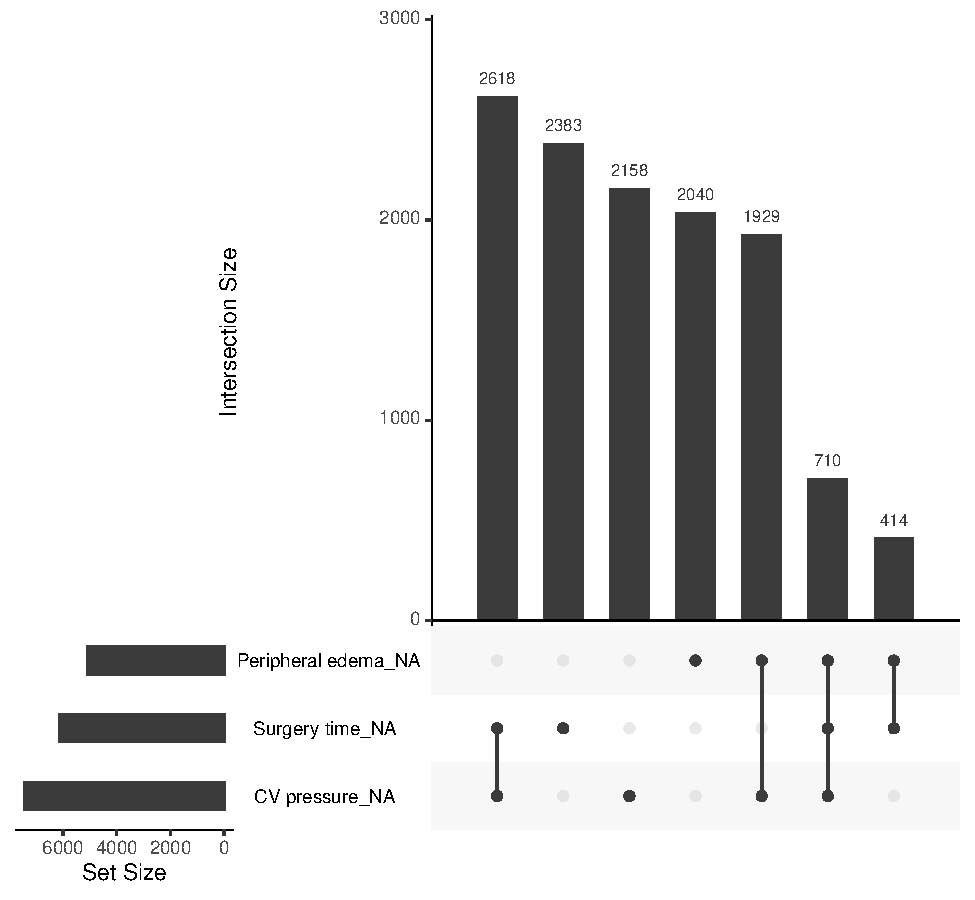
\includegraphics{doc_arxiv_files/figure-latex/upset-1} 

}

\caption{An upset plot showing three variables from the INTERMACS registry and all combinations of missing patterns. The bottom left plot shows the number of missing values for each variable, separately. The top right plot shows the number of missing values for each combination of the three variables. For example, there were 2,618 rows in the overall INTERMACS data where both CV pressure and surgery time were missing.}\label{fig:upset}
\end{figure}

\clearpage

\begin{figure}

{\centering 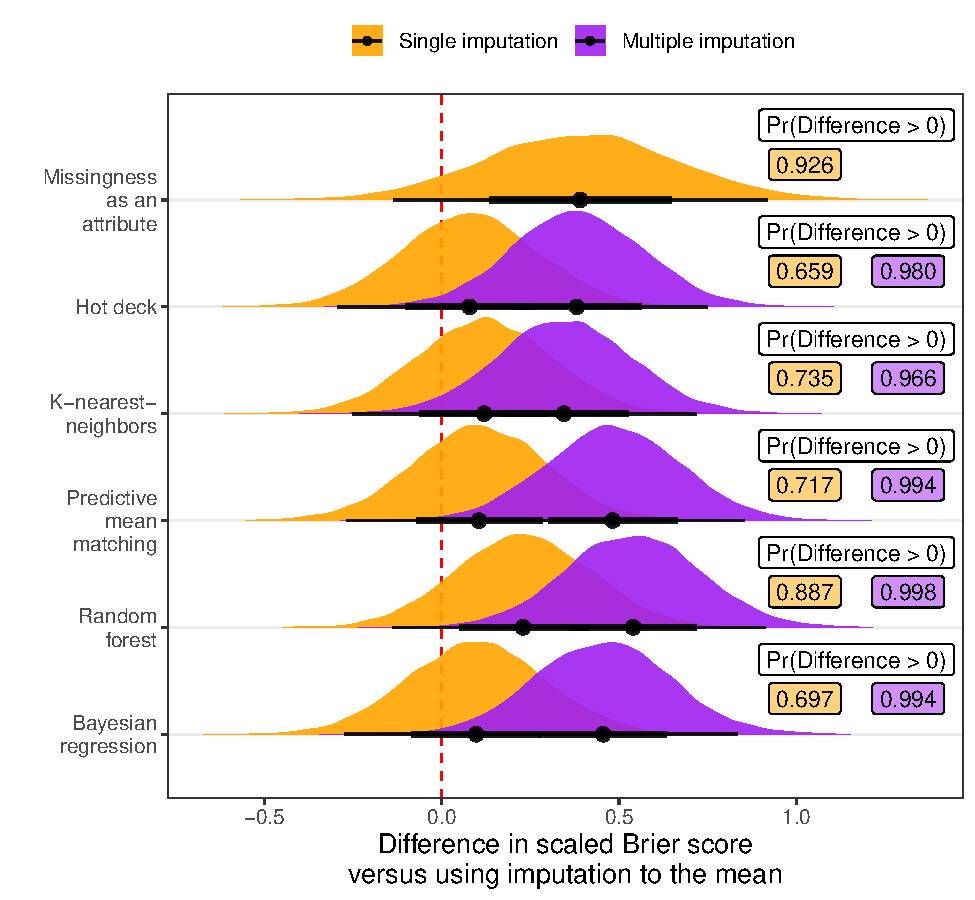
\includegraphics{doc_arxiv_files/figure-latex/fig_md_strat_infer_ipa-1} 

}

\caption{Posterior distribution of differences in scaled Brier score values relative to imputation to the mean when different imputation strategies are applied before fitting a risk prediction model. Results are aggregated over scenarios where the outcome is mortality and transplant and the amount of additional missing data is 0\%, 15\%, or 30\%. Posterior probability that the difference in scaled Brier score exceeds 0, indicating an improvement in overall model accuracy, is printed to the right of each distribution. Each multiple imputation strategy and single imputation with missingness incorporated as an attribute had over 90\% posterior predicted probability of increasing the scaled Brier score versus using imputation to the mean.}\label{fig:fig_md_strat_infer_ipa}
\end{figure}

\clearpage

\begin{figure}

{\centering 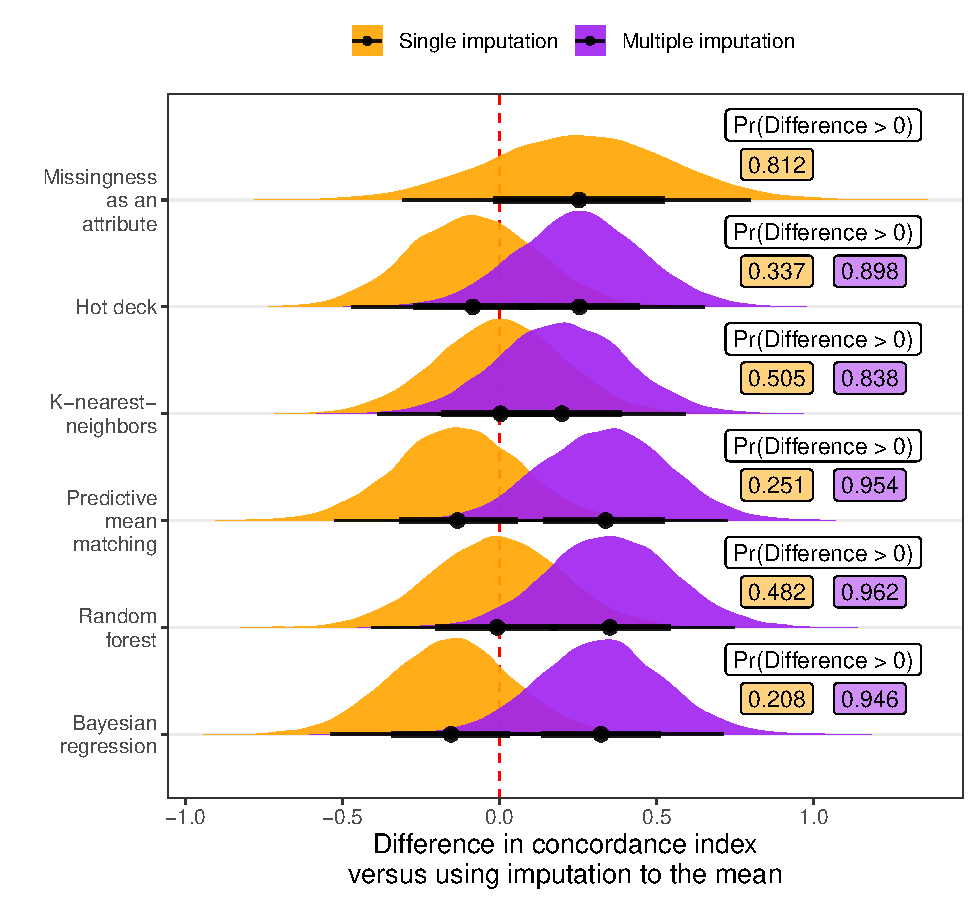
\includegraphics{doc_arxiv_files/figure-latex/fig_md_strat_infer_auc-1} 

}

\caption{Posterior distribution of differences in concordance index values relative to imputation to the mean when different imputation strategies are applied before fitting a risk prediction model. Results are aggregated over scenarios where the outcome is mortality and transplant and the amount of additional missing data is 0\%, 15\%, or 30\%. Posterior probability that the difference in concordance index exceeds 0, indicating an improvement in model discrimination, is printed to the right of each distribution. Multiple imputation with predictive mean matching, random forests, and Bayesian regression each had over 90\% posterior predicted probability of increasing the concordance index versus using imputation to the mean.}\label{fig:fig_md_strat_infer_auc}
\end{figure}

\clearpage

\begin{figure}

{\centering 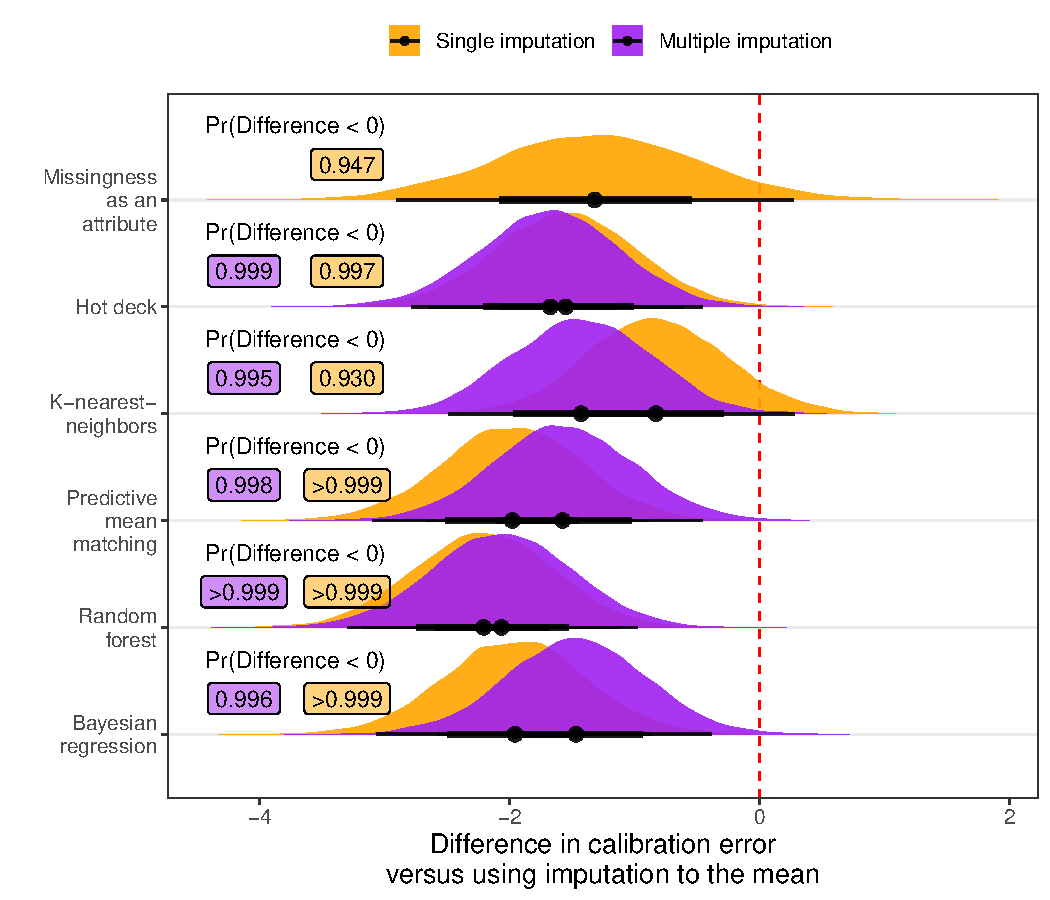
\includegraphics{doc_arxiv_files/figure-latex/fig_md_strat_infer_cal_error-1} 

}

\caption{Posterior distribution of differences in calibration error values relative to imputation to the mean when different imputation strategies are applied before fitting a risk prediction model. Results are aggregated over scenarios where the outcome is mortality and transplant and the amount of additional missing data is 0\%, 15\%, or 30\%. Posterior probability that the difference in calibration error is less than 0, indicating an improvement in model calibration, is printed to the right of each distribution. Every imputation strategy evaluated had over 90\% posterior predicted probability of improving model calibration versus using imputation to the mean.}\label{fig:fig_md_strat_infer_cal_error}
\end{figure}

\clearpage

\bibliographystyle{unsrt}
\bibliography{references.bib}


\end{document}
